\section{Methodology}
\label{sec:method}
\subsection{Low-rank Matrix Factorization (LMF) for Compressing Neural Models}
\label{sec:method_svd}
Low-rank Matrix Factorization (LMF) exploits latent structure in the data to obtain a
compressed representation of a matrix. It does so by factorization of the
original matrix into low-rank matrices. For a full rank matrix $W
\in R^{m\times n}$ of rank $r$, there always exists a factorization $W=W_a
\times W_b$ where $W_a \in \mathbb{R}^{m \times r}$ and $W_b \in \mathbb{R}^{r \times n}$. Singular Value Decomposition (SVD) \cite{golub1970singular} achieves this factorization as follows:
\begin{equation}\label{eq1}
W_{m\times n} = U_{m\times m}\Sigma_{m\times n}V^{t}_{n\times n} 
\end{equation}
where $\Sigma_{m\times n}$ is a diagonal rectangular matrix of singular values of descending
magnitude.  We can compress the matrix by choosing the $k$ largest singular
values, with $k<m$ and $k<n$. For low rank matrices, the discarded singular values will be zero or small, therefore the following will approximately hold:
\begin{equation}\label{eq2}
W_{m\times n} \approx U_{m\times k}\Sigma_{k\times k}V^{t}_{k\times n} \newline
%= U_{m\times k}N_{k\times n}
\end{equation}

Therefore, the original matrix $W$ is compressed into two matrices:
\begin{equation}\label{eq3}
W_a = U \in \mathbb{R}^{m \times k} \newline
\end{equation}
\begin{equation}\label{eq4}
W_b = \Sigma_{k\times k}V^{t}_{k\times n} \in \mathbb{R}^{k \times n}
\end{equation}

The number of parameters are reduced from $m \times n$ to $k\times(m +
n)$. Therefore, to achieve a $p$ fraction parameter reduction, $k$ should be
selected as:
\begin{align}\label{eq5}
(p \times m \times n) =  k \times (m + n) \notag \\
%\end{equation}
%\begin{equation}\label{eq6}
k = \floor* {\frac{pmn}{m + n}} ;  k \in \mathbb{Z}^{+} 
\end{align}

The value $k$ can be varied  depending on the desired compression fraction $p$ as long as $k \geq 1$. In practice, being able to decide an arbitrary compression fraction $p$ is an attractive property for model compression, since it allows choosing compression rates based on the accuracy-memory trade-offs of a downstream application. 
%Standard quantization techniques do not offer this flexibility, as they typically allow compression fractions of $1/2$ or $1/4$ (corresponding to 16-bit or 8-bit quantization from 32-bits typically).
The low rank matrix factorization operation is illustrated in
Figure~\ref{fig:decomposition}, where a single neural network matrix (layer) is
replaced by two low rank matrices (layers).
\begin{figure}[th]
	\centering
	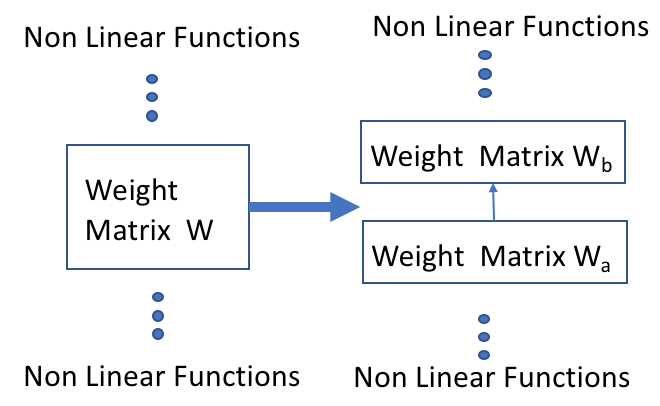
\includegraphics[width=0.35\textwidth]{breakdnn.png}
	\caption{Replacing one neural network matrix with two low rank matrices}
	\label{fig:decomposition}
\end{figure}
\vspace{-8 pt}
\subsubsection{Compressing the Word Embedding Matrix }
%% Needs Major Revision 
For NLP tasks, typically the first layer of the neural model consists of an
embedding lookup layer that maps the words into real-valued vectors for
processing by subsequent layers. The words are indices $i$ of a word dictionary
of size $D$ while the word embeddings are vectors of size $d$. This corresponds
to a lookup table $E(i) = W_i$ where $W \in \mathbb{R}^{d \times |D|}$. The word
embeddings are often trained offline on a much larger corpus, using algorithms
like Word2Vec, GloVe etc, and are then fine-tuned during training on the downstream NLP task.  Our method 
decomposes the embedding layer in an online fashion during training using eq.(\ref{eq5}).
$W_a$ becomes the new embedding layer and $W_b$ becomes the next layer. Continuing backpropagation over this new network struture finetunes the low rank embedding space and regains any accuracy loss within a few epochs.
%the low rank embedding space to finetune the embedding
%weights based for the task in hand and regain lost accuracy.
%We use this new network struture to continue training and fine tune the network
%weights on the downstream task.
%% and carry on
%% training letting backpropagation over the low rank embedding space to finetune
%% the embedding weights based for the task in hand and regain lost accuracy.
% Discuss in Result :As discussed earlier (Sec: \ref{contribution}) and backed by emperical evidence presented in ( Sec: \ref{results:sst}) we see significant accuracy improvement over offline embedding compression. 
%Our method applies \ref{eq5} on the embedding layer of the deep NLP model and decomposes it into two low rank matrices like \ref{eq3} and \ref{eq4} We use  
%The embedding layer often corresponds to the largest matrix in an NLP model,
%because the vocabulary size $D$ can be of the order of hundred of thousand
%words, depending on the application, often resulting in embedding matrix $W$
%with millions of parameters. Therefore, in this work, we focus on compressing
%the input embedding matrix, decomposing it into a low rank embedding and a weight layer through  although SVD could be applied for compressing any
%other matri\ref{}of the neural model
%When we are compressing embedding m is the vocabulary size which tends to be fairly large and n is the fixed embedding dimension thus we can safely assume $mn >> (m+n)$. 
%\cite{sainath2013low} \cite{lu2016learning} trained two DNN side-by-side where all 
%to project the weight layers of a DNN onto lower dimensional subspace to reduce the model size for a Speech task. They showed that these bottleneck network is a good approximation and achieves compression with small loss in accuracy. \cite{zhang2014extracting} used a similar idea of projecting the weight matrix onto lower dimensional subspace using SVD.    
\subsection{Cyclically Annealed Learning Rate }
\label{subsec:method_training_scheme}
Due to the non-convex nature of the optimization surface of DNNs, gradient based algorithms like stochastic gradient descent (SGD) are prone to getting trapped in suboptimal local minima or saddle points. Adaptive learning rates like Adam~\cite{kingma2014adam} and Adagrad ~\cite{duchi2011adaptive} try to solve this problem by tuning learning rate based on the magnitude of gradients. While in most cases they find a reasonably good solution, they usually can't explore the entire gradient landscape. \cite{bergstra2012random,loshchilov2016sgdr} indicates periodic random initialization or warm restarts often helps in better exploration of the landscape while \cite{smith2017cyclical} showed that letting the learning rate(LR) vary cyclicaly (Cyclic learning rate(CLR)) helps in faster convergence.  
In this work we further refine CLR and propose a simulated annealing inspired LR update policy we call Cyclically Annealed Learning
Rate~(CALR). CALR is described in algorithm (\ref{alg:Exp_clr}) and Fig. \ref{modified_clr}. In addition to varying LR in a CLR style triangular windows(Fig.~\ref{clr}), CALR expontentially decays the upper bound $LR_{UB}$ of the triangular window from its initial value. When the learning rate decreases to a lower bound $LR_{LB}$, we increase the upper bound to its initial value $LR_{UB}$ and continue with the LR updates. This exponential decay ensures slow steps on the optimization
landscape. Intuitively, the proposed warm restarts, motivated by simulated annealing, make
CALR more likely to escape from local minima or saddle points and enables better
exploration of the parameter space.  CALR should have similar but less
aggressive effect as random initialization or warm restarts of LR. While exponentially decayed small
cyclic windows let CALR carefully explore points local to the current solution,
cyclic temperature increase helps it jump out and explore regions around other
nearby local minima. We verified this intuition empirically for our
classification experiments~(Table~\ref{results:uncompressed}, Secton \ref{sec:experiments_uncompresed}), where CALR was
able to achieve further improvement compared to CLR and Adagrad.

%In this work, we extend CLR and propose an LR policy, inspired from simulated annealing, that we call Cyclically Annealed Learning Rate~(CALR). CALR is described in algorithm (\ref{alg:Exp_clr}) and Fig. \ref{modified_clr}.  In addition to using a CLR style triangular window, in CALR we  expontentially decay the upper bound $LR_{UB}$ of the triangular window from its initial value. When the learning rate decreases to a lower bound $LR_{LB}$, we increase the upper bound to its initial value $LR_{UB}$ and continue with the learning rate schedule as before. This exponential decay ensures slow steps on the optimization landscape. Intuitively, the proposed warm restarts, motivated by simulated annealing, make CALR more likely to escape from local minima or saddle points and enables better exploration of the parameter space.  CALR should have similar but less aggressive effect as random initialization or warm restarts of LR \cite{loshchilov2016sgdr,bergstra2012random}. While exponentially decayed small cyclic windows let CALR carefully explore points local to the current solution, cyclic temperature increase helps it jump out and explore regions around other nearby local minima. We verified this intuition empirically for our classification experiments~(Table~\ref{results:uncompressed}, Secton \ref{sec:experiments_uncompresed}), where CALR was able to achieve further improvement compared to CLR and Adagrad.

%\cite{smith2017cyclical} suggest that
 %letting the learning rate~(LR) vary within a range cyclically is likely to
% find better solutions, they call this Cyclic Learning Rate~(CLR) (Fig.~\ref{clr}).
 \begin{figure}[!htb]
 	%\minipage{0.2365\textwidth}	
 	\begin{subfigure}{.23\textwidth}
 		\centering
 		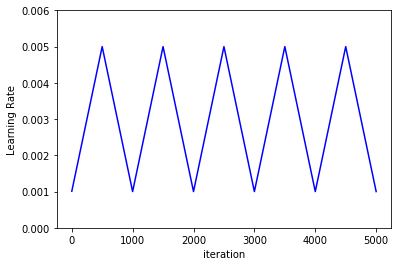
\includegraphics[width=\linewidth]{CLR.png}\caption{CLR}	\label{clr} 
 	\end{subfigure}
 	%\caption{}
 	%\endminipage\hfill
 	%\minipage{0.2365\textwidth}
 	\begin{subfigure}{.23\textwidth}	
 		\centering
 		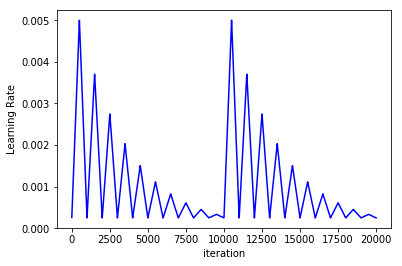
\includegraphics[width=\linewidth]{Modified_CLR.png}\caption{CALR}	\label{modified_clr} 
 		%\caption{}\label{2b}
 		%\endminipage\hfill
 	\end{subfigure}
 	\caption{Comparison of CLR and CALR update Policy }
 \end{figure}
\begin{algorithm}
	\caption{Cyclically Annealed Learning Rate Schedule}\label{alg:Exp_clr}
	\begin{algorithmic}[1]
		\Procedure{CALR}{Iteration, Step Size, $LR_{LB}$, $LR_{UB}$}
		\State $LR_{UB} \gets LR_{UB} (init) $
		\State $LR_{LB} \gets LR_{LB} (init) $
		%\State $LR_{LB} \gets LR_{UB} (init) \times \exp(Decay)^{ResetStep}$
		%\Comment{This ensures if $LR_{UB}$ is decayed exponentially by the Decay Rate it will become $\leq LR_{LB}$ after ResetStepSize Epochs}
		\ForEach{EPOCH}
		\State $LR_{UB} \gets LR_{UB}\times \exp(Decay)$
		\If{$LR_{UB} \leq LR_{LB}$}
		\State $LR_{UB} \gets LR_{UB} (init)$
		%\State $LR_{LB} \gets LR_{UB} (init) \times \exp(Decay)^{ResetStep}$
		\EndIf
		\ForEach{Training BATCH}
		\State LR $\gets$ CLR(Iteration,StepSize,$LR_{LB}, LR_{UB}$)
		\EndFor
		\EndFor
		\Return $LR$
		\EndProcedure
	\end{algorithmic}
	\begin{algorithmic}[1]
		\Procedure{CLR}{Iteration, Step Size, $LR_{LB}$, $LR_{UB}$}
		\newline
		\Comment{this procedure implements a triangular window of width StepSize and height $LR_{UB} - LR_{LB}$}
		\State $Bump\gets \frac{LR_{UB} - LR_{LB}}{Step Size}$
		\State $Cycle \gets (Iteration) \bmod (2 \times StepSize)$
		\If{$Cycle < StepSize$}
		\State $LR \gets LR_{LB} + (Cycle \times Bump)$
		\Else 
		\State $LR \gets LR_{UB} - (Cycle - StepSize)\times Bump$
		\EndIf
		\Return $LR$
		\EndProcedure
	\end{algorithmic}
\end{algorithm} 

%In this work we further extend CLR and propose an exponentially decayed and iteratively boosted version of the cyclic learning rate schedule, that we call 
%Wiggly Triangular Learning Rate (WTLR). WTLR is ploted in
%Fig. \ref{modified_clr}, and described in Algorithm 1. At each epoch we
%decay the upper bound $LR_{UB}$ of the triangular window by an exponential
%factor which results in an exponentially decayed version of CLR. As a result of
%this exponential decay when the learning rate decreases to a lower bound
%$LR_{LB}$, we increase the upper bound to its initial value $LR_{UB}$ and
%continue with the learning rate schedule as before. The intuition is loosely
%inspired from simulated annealing.  We think that this iterative boosting is
%equivalent to changing the temperature and similar to simulated annealing helps
%the optimizer to escape from local minima or saddle points while it enables
%better exploration of the parameter space \cite{bibid}.  We verified this
%intuition empirically for our classification experiments in Section
%\ref{sec:experiments}, where our proposed WTLR schedule achieved further
%improvement compared to CLR and Adam.
%To effectively train our networks we experimented with different learning rate
%schedules including Adam\cite{kingma2014adam}, Adagrad ~\cite{duchi2011adaptive} and Cyclic
%Learning Rates (CLR) \cite{smith2017cyclical}.
%and we
%propose a novel extension of the CLR scheme. CLR was introduced by
%\cite{smith2017cyclical} who argued that letting the learning rate of gradient
%descent algorithms vary within a range cyclically (Fig. \ref{clr}) yields a
%better optimization compared to popular adaptive learning schedules like ADAM
%\cite{kingma2014adam}, Adadelta \cite{zeiler2012adadelta}. %CLR learning rates
%are plotted in Fig. \ref{fig:clr}.
%We think that this iterative boosting is equivalent to changing the temperature and similar to simulated annealing helps
%the optimizer to escape from local minima or saddle points while it enables
%better exploration of the parameter space \cite{bibid}.  We verified this
%intuition empirically for our classification experiments in Section
%\ref{sec:experiments}, where our proposed WTLR schedule achieved further
%improvement compared to CLR and Adam.
%Training a DNN is challenging due to the inherent non-convex nature of the loss function topology. Gradient Descent(GD) based algorithms though have been proven to be extremely effective but are prone to getting stuck in the saddle point plateaus of the non-convex optimization landscape \cite{dauphin2015equilibrated}. 
%\begin{figure}[h] 
%	\centering 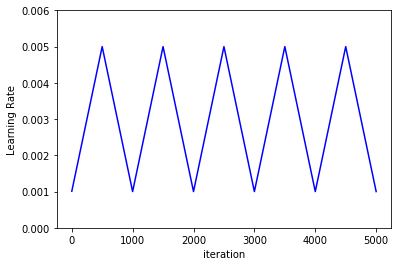
\includegraphics[width=\linewidth]{CLR.png}
%	\captionof{figure}{\normalsize Triangular Window Cyclic Learning Rate \label{plot:clr}}
%	%% \vspace{-0.4cm}
%\end{figure}
%\begin{figure}[h]
%	\centering 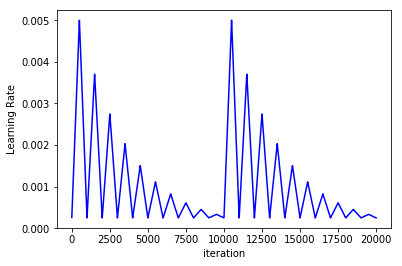
\includegraphics[width=\linewidth]{Modified_CLR.png}
%	\captionof{figure}{\normalsize Proposed Modified Cyclic Learning Rate \label{plot:modifier_clr}}
%	%% \vspace{-0.4cm}
%\end{figure}


%\begin{figure}[h]
%       \centering
%        \begin{subfigure}[b]{0.45\textwidth}
%                \centering
%                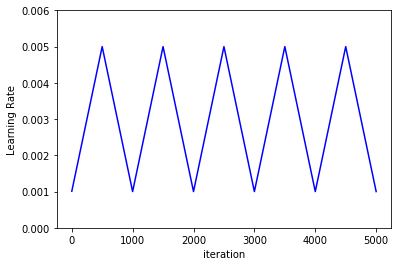
\includegraphics[width=.7\linewidth]{CLR.png}
%                \caption{Triangular Cyclic Learning Rate (TCLR)}
%                \label{fig:clr}
%        \end{subfigure}
%        \begin{subfigure}[b]{0.45\textwidth}
%                \centering
%                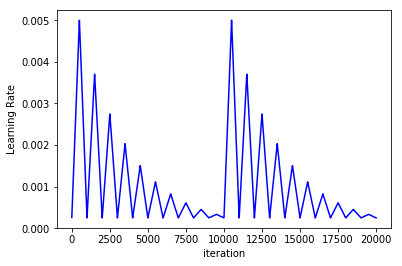
\includegraphics[width=.7\linewidth]{Modified_CLR.png}
%                \caption{Exponentially Decayed Triangular Cyclic Learning Rate (WTLR)}
%                \label{fig:modified_clr}
%        \end{subfigure}%
%        \caption{TCLR and the proposed WTLR schedules}
%        \label{fig:sst2_plots}
%\end{figure}
\subsection{Baselines}
\label{subsec:method_baselines}
We compare our proposed method with two commonly baselines for neural model compression.
%% We compare our proposed method with two baselines that has been used in prior state-of-art method for compressing embedding space of deep NLP models.
\subsubsection{Fixed Point Weight Quantization (Baseline 1)}
We compare our approach with widely used post-training fixed point quantization
\cite{bengio2013estimating,gong2014compressing} method where the weights are
cast into a lower precision. This requires less memory to store them and doing low
precision multiplications during forward propagation improves inference latency.
%Several model weight quantization algorithms have been proposed in the
%literature, here we use tensorflow's ~\cite{abadi2016tensorflow} native
%quantization as our second baseline.
%[@Anish describe the details of the quantization baseline]
\subsubsection{Offline Embedding Compression (Baseline 2)}
In this set of baseline experiments we compress the embedding matrix in a
similar way using SVD but we do it as a preprocessing step similar to
~\cite{raunak2017effective,joulin2016fasttext}. For example, if we have a 300
dimensional embedding and we want a 90\% parameter reduction we project it onto
a 30 dimensional embedding space and use this low dimensional embedding to train
the NLP model.





